\section{Sampling Update Patterns}
\label{sampling}
Updates can affect the three classes of materialized views in different ways, making sampling challenging. 
%and our sample should represent how the update will affect the materialized view.
We describe this process as sampling the ``update pattern".
In this section, we discuss how to efficiently sample update patterns for different types of views.
We first formalize the update patterns in Section~\ref{subsec:pattern}, and then present scalable sampling techniques in Section~\ref{subsec:sample-pattern}. 
We also analyze the costs and overheads of our methods.

\begin{figure}[tup]
\centering
 \hspace*{-2em}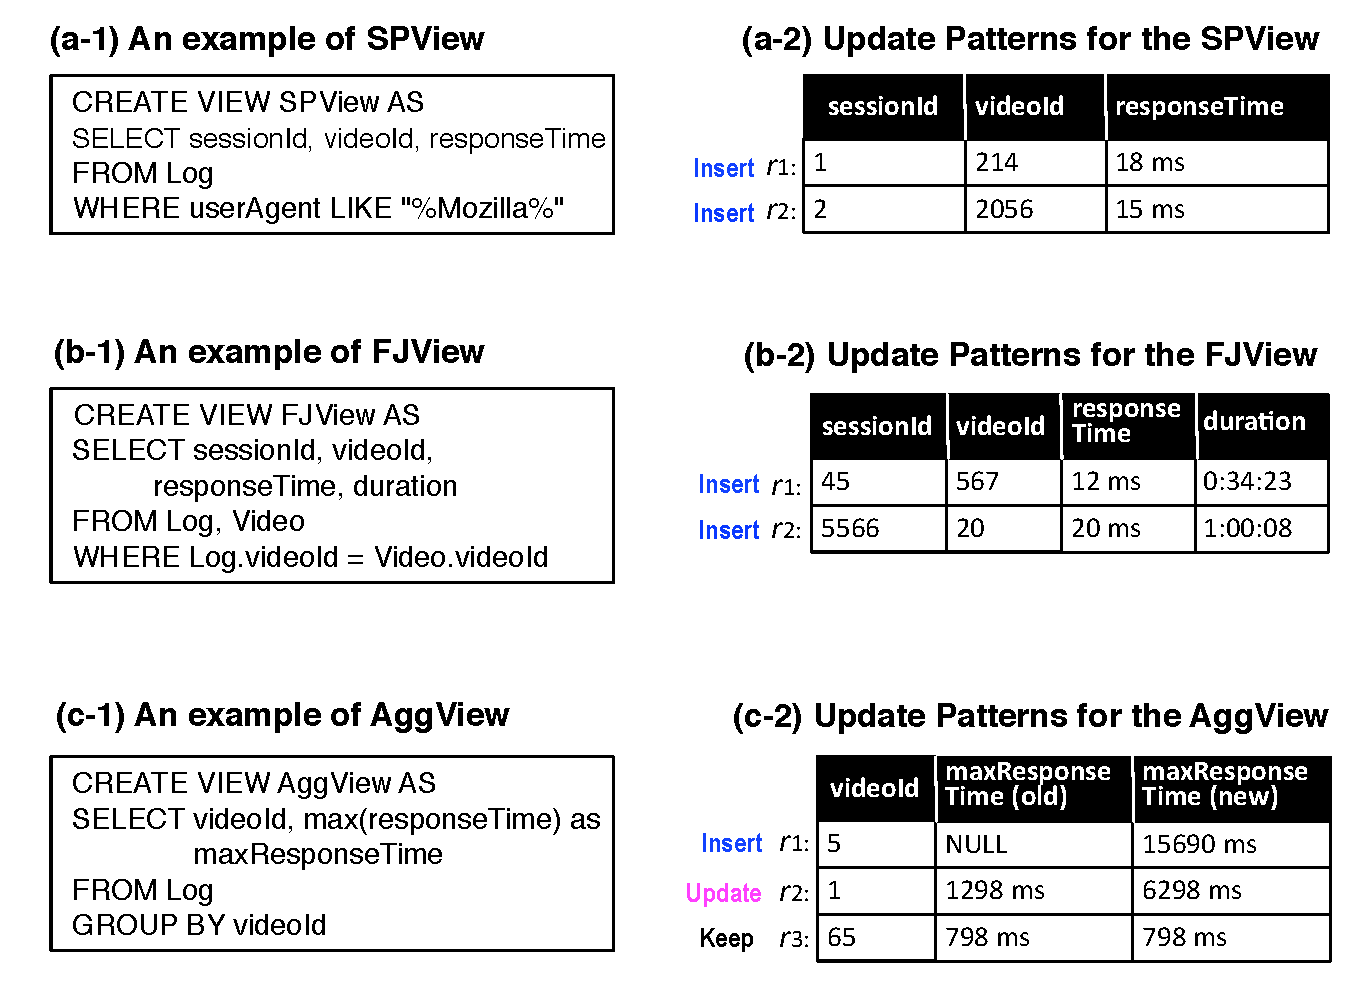
\includegraphics[scale=0.38]{figs/update-pattern-new.pdf}\vspace{-1em}
 \caption{Illustration of the update patterns for \spview and \fjview and \aggview.}\label{fig:update-pattern}\vspace{-1em}
\end{figure}

\begin{table*}\renewcommand{\arraystretch}{1.2}

\caption{Cost comparison between incremental view maintenance and update-pattern sampling.}\label{tbl:cost-analysis} \small \centering
%\begin{tabular}[t]{|c@{\::\:}l@{\:,\:}l@{\:,\:}r|}
%\begin{tabular}[t]{|@{\:\:}l@{\:\:}||@{\:\:}r@{\:\:}|@{\:\:}r@{\:\:}|@{\:\:}r@{\:\:}|}
\begin{tabular}[t]{|l||c | c||c|c||c|c|}
  %\multicolumn{4}{c}{\normalsize {(a) $\ars$}} \\ \hline
  %\multicolumn{4}{|c|}{A set $\Lambda$ of $\ar$s} \\ \hline\hline
   \hline
   & \multicolumn{2}{c||}{\bf{\spview}}  & \multicolumn{2}{c||}{\bf{\fjview}}  & \multicolumn{2}{c|}{\bf{\aggview}}  \\ \cline{2-7} 
   &  \bf{Maintenance} & \bf{Sampling}  &  \bf{Maintenance}  &  \bf{Sampling} & \bf{Maintenance} & \bf{Sampling} \\ \hline \hline
   
  %\bf{Scan of Updates} & $\mathcal{O}$($n\cdot \textrm{cost}_{read}$) & $\mathcal{O}$($n\cdot \textrm{cost}_{read}$) & $\mathcal{O}$($n\cdot \textrm{cost}_{read}$) & $\mathcal{O}$($n\cdot \textrm{cost}_{read}$) & $\mathcal{O}$($n\cdot \textrm{cost}_{read}$)  & $\mathcal{O}$($n\cdot \textrm{cost}_{read}$) \\ \hline
  \bf{Delta View} & $\textrm{cost}_{pred}(n)$ & \specialcell{$\textrm{cost}_{rand}(n)$ + \\$ \textrm{cost}_{pred}(\ratio \cdot n)$}  & $\textrm{cost}_{join}(n)$ & \specialcell{$ \textrm{cost}_{rand}(n)$ + \\ $\textrm{cost}_{join}(\ratio \cdot n)$} &
  \specialcell{$\textrm{cost}_{group}(n)$ \\+ $\textrm{cost}_{agg}(\delta_{v})$} &
   \specialcell{$\textrm{cost}_{hash}(n)$ + \\$\textrm{cost}_{group}(\ratio \cdot n)$ + \\ $\textrm{cost}_{agg}(\ratio \cdot \delta_{v})$}        \\ \hline
  \bf{Refresh}    & $\textrm{cost}_{write}(\delta_v)$ & $\textrm{cost}_{write}(\ratio \cdot \delta_v)$  & $\textrm{cost}_{write}(\delta_v)$ & $\textrm{cost}_{write}(\ratio \cdot \delta_v)$ &  $\textrm{cost}_{apply}(\delta_v)$ & $\textrm{cost}_{apply}(\ratio \cdot \delta_v)$\\ \hline
\end{tabular}
\end{table*}


\subsection{Update Patterns}\label{subsec:pattern}
An \emph{update pattern} represents how an update to a base table affects a materialized view derived from that table.
We define this information to be such that if we took a 100\% sample the information would be sufficient to transform the stale view to the corresponding up-to-date view exactly. 
In our model, there are three possible update patterns. (1)~Insert a new row into a view;
(2)~Update attribute values of an existing row in the view; (3)~Keep the view unchanged.
Figure~\ref{fig:update-pattern} illustrates the update patterns of the three types of views supported by our system.

For \spview, the only possible updates to the view are inserting new rows.  
For instance, Figure~\ref{fig:update-pattern}(a-1) shows an example of \spview. When the base table \tbl{Log} is updated, there might be some new rows whose \field{userAgent} field contains "Mozilla", which should be added into the \spview accordingly. Figure~\ref{fig:update-pattern}(a-2) illustrates the update patterns for the \spview. The figure means that in order to obtain the up-to-date \spview, we should insert $r_1$ and $r_2$ into the original \spview.

For \fjview, similar to \spview, its update patterns only involve insertion. For instance, Figure~\ref{fig:update-pattern}(b-1) shows an example of \fjview. When the base tables, \tbl{Log} or \tbl{Video} are updated, there might be some new rows that satisfy the join condition, which should be added into the \fjview accordingly. Figure~\ref{fig:update-pattern}(b-2) illustrates the update patterns for the \fjview. The figure means that we should insert $r_1$ and $r_2$ into the original \fjview to obtain the up-to-date \fjview.

For \aggview, the updates could be inserting a new group, updating the aggregation attribute values of an existing group, or keep the view unchanged. 
For instance, Figure~\ref{fig:update-pattern}(c-1) shows an example of \aggview and Figure~\ref{fig:update-pattern}(c-2) illustrates the update patterns for the \aggview. In the figure, ``Insert $r_1$" indicates that the group-by key, ``videoId = 5", does not exist in the original view, and we need to insert this new group into the view; ``Update $r_2$" indicates that the group-by key, ``videoId = 1", is already in the original view, and we should update the aggregation attribute value (i.e., \field{maxResponseTime}) of the group from 1298 ms to 6298 ms; ``Keep $r_3$" indicates that the group-by key, ``videoId = 65", is already in the original  view, and we do not need to change the aggregation attribute value of the group.    



\subsection{Sampling Techniques for Update Patterns}\label{subsec:sample-pattern}
Modeling updates to the base table in terms of update patterns does not change the expense of incremental view maintenance.
It does, however, give us a logical unit to sample and in this section, we describe how 
our system only maintains a random sample of the update patterns.
As our earlier analysis of the update patterns suggests, our sampling techniques for each type of materialized view are slightly different.

\subsubsection{Select-Project and Foreign-Key Join Views}
Consider a base table $T$ and the corresponding insertion table $\triangle T$. Given a \spview defined on the table, its full update patterns involve the inserted records of $\triangle T$ that satisfy the predicate of the \spview. To sample the update patterns (e.g., at a sampling ratio of $\ratio = 5 \%$), we randomly select 5\% records from $\triangle T$, and then keep the records that satisfy the view's predicate as a sample. 

\sloppy

For a given \fjview, let $T$ be the fact table, and $T_1, T_2, \cdots, T_k$ be the dimension tables. The update patterns of the \fjview involve the inserted records of $\triangle T \bowtie (T_1+\triangle T_1) \bowtie (T_1+\triangle T_1) \cdots \bowtie (T_k+\triangle T_k)$ that satisfy the predicate of the \fjview\footnote{Due to foreign-key integrity constraints, it is guaranteed that the join result of $T \bowtie \triangle T_i ~(1\leq i \leq k)$ is empty.}. Similar to \spview, to sample the update patterns (e.g., $\ratio= 5 \%$), we first randomly select 5\% records from $\triangle T$, and then join the selected records with the up-to-date dimension tables (i.e., $T_i + \triangle T_i ~(1\leq i \leq k)$), and finally return as a sample the joined records that satisfy the \fjview's predicate. 

\fussy



\vspace{.5em}


{\noindent \bf Cost Analysis.} Let $n = |\triangle T|$ be the number of inserted records, $v$ be the cardinality of the stale view, $\delta_v$ be the cardinality of the delta view, and $\ratio$ be the sampling ratio. Table~\ref{tbl:cost-analysis} compares the cost of our update-pattern sampling techniques (denoted by Sampling) with the corresponding cost of incremental view maintenance (denoted by Maintenance). The table does not include the I/O cost of loading the updates into memory since in both Sampling and Maintenance we only need to load the updates once and amortize that I/O cost over all views.

%Both incremental view maintenance and our proposed solution require at least one scan of the inserted records. But note that in both solutions we can load the updates into memory once and amortize that I/O cost over all views.



\vspace{-.5em}

\begin{itemize} %[leftmargin=5.5mm]
\item \underline{Delta View.} For \spview and \fjview, incremental view maintenance has the processing cost of $\cost_{pred}(n)$ and $\cost_{join}(n)$, respectively, since they have to evaluate the predicate or the join for all $n$ inserted records. Our sampling approach can reduce this number to $\ratio \cdot n$ as we only need to evaluate this on our sample. The additional overhead of sampling is to generate $n$ random numbers, i.e., $\cost_{rand}(n)$. \vspace{-0.5em}
\item \underline{Refresh.} For \spview and \fjview, incremental view maintenance has to insert $\delta_v$ rows into the original view while we have to insert only $\ratio \cdot \delta_v$ records into the sample of update patterns. %\reminder{Move this to ourlier indexing section? ``If there is an outlier index, this cost increases to $\ratio\delta_v + l$"} 
\end{itemize}
\vspace{-.5em}

From the above analysis, we can see that for \spview and \fjview, when the predicate or the join is expensive to evaluate, our sampling techniques require much less cost than incremental view maintenance. For example, if the time of generating $n$ random numbers is negligible, we can save the cost of incremental view maintenance by 20 times for the sampling ratio of $\ratio = 5 \%$.

\subsubsection{Aggregation View}
The update patterns for an \aggview contains the update information for each existing group in the view as well as newly inserted groups. 
To sample the update patterns, we seek to maintain the update patterns for a sample of groups. That is, for the existing group keys in the \aggview, we keep track of the update patterns for a sample of them; for the newly inserted group keys, we choose a sample of them to maintain. 

To implement this idea, we incorporate hashing into our sampling techniques. The basic idea is similar to hash partitioning, where a sample can be thought as a data partition. Specifically, we define a hash function, $\hashfunc{\cdot}$, which takes a single group key as an input and outputs a uniform random number in the range of [0, 1]. We only maintain the update patterns for the group keys such that
\begin{equation}\label{eq:hash}
\hashfunc{\textrm{``group key"}} \leq \ratio.
\end{equation}
Obviously, the maintained group keys are a random sample of all the group keys with the sampling ratio of~$\ratio$.
With this hash-based sampling technique, we can easily devise an efficient update-pattern sampling approach for an \aggview. 


To better understand the approach, we first introduce how to obtain the full update patterns of an \aggview. The idea is the same as incremental view maintenance, which first computes a delta \aggview by executing the \aggview definition on an insertion table and then obtains the full update patterns by refreshing the \aggview with the delta \aggview. Similarly, to sample the update patterns, we first compute a delta \emph{sample} \aggview by executing the \aggview definition on the  records of an insertion table that satisfy $\hashfunc{\textrm{``group key"}}~\leq~\ratio$, and then obtains the \emph{sample} update patterns by refreshing the \emph{sample} \aggview with the delta \emph{sample} \aggview. 

%Given an insertion table $\triangle T$, since we are only interested in the update patterns for a sample of group keys, we execute the view definition on the records in $\triangle T$ that satisfy the Equation~\ref{eq:hash}


%to obtain $S_{V}$'s update patterns w.r.t $\triangle T$, we first compute a \emph{delta sample \aggview} by executing the view definition on the records in $\triangle T$ that satisfy the Equation~\ref{eq:hash}, and then obtain $S_{V}$'s update patterns by applying the delta sample \aggview to~$S_{V}$. 

\vspace{.5em}
{\noindent \bf Cost Analysis: }
 Table~\ref{tbl:cost-analysis} shows the cost comparison between our update-pattern sampling and incremental view maintenance.
\vspace{-0.5em}
\begin{itemize}
%\item Scan of Updates.
%As in \spview and \fjview, both incremental view maintenance and our proposed solution require at least one scan of the inserted records, and in both solutions we can load the updates into memory once and amortize that I/O cost over all views. \vspace{-0.5em}
\item \underline{Delta View.} For \aggview, incremental view maintenance has a grouping cost of $\cost_{group}(n)$ as well as an aggregation cost of $\cost_{agg}(\delta_v)$ where aggregates for each of the groups have to be maintained. In contrast, since we only maintain the update patterns for a sample of groups, we can reduce the grouping cost to $\cost_{group}(\ratio \cdot n)$ and the aggregation cost to $\cost_{group}(\ratio \cdot \delta_v)$. The additional overhead of sampling is to evaluate $\hashfunc{\cdot}$ for each inserted record, i.e., $\cost_{hash}(n)$.  \vspace{-0.5em}
%Furthermore, in a distributed environment, there are potentially additional communication costs as the updates may not be partitioned by the group-by key. \vspace{-0.5em}
\item \underline{Refresh.} Compared to \spview and \fjview, the refresh cost of \aggview is a little bit more complicated as we have a combination of insertions into the view and updates to the view. 
Incremental view maintenance has to apply $\delta_v$ records to the entire view while our sampling approach only needs to apply $\ratio \cdot \delta_v$ records to the sample view. 
If there is an index in the view, we can 
determine which records are new insertions and which correspond to existing records in constant time. Therefore, our sampling technique can reduce the refresh cost from $\cost_{apply}(\delta_v)$ to $\cost_{apply}(\ratio\cdot \delta_v)$.

\vspace{-0.25em}

%The costs become higher in a distributed environment as we need to consider communication and query processing engines that rely on partitioned joins rather than indices.
%For aggregation views, we want to partition the data by the group-by key.
%This allows a partitioned join which only requires communication (a shuffle operation) of the delta table.
%Therefore, in incremental maintenance we have to communicate $\delta_v$ rows while our solution requires $\ratio \cdot \delta_v$ rows. 
\end{itemize}

Similar to the analysis results of \spview and \fjview, our sampling techniques can save the cost by a factor of $1/\ratio$ in almost every stage of incremental view maintenance. The only additional overhead is to compute a hash value for each inserted record (i.e., $\cost_{hash}(n)$). However, as shown in our experiments (Section~??), even with the additional overhead, our sampling techniques can still run orders of magnitude faster than incremental view maintenance. %\reminder{I remove the cost analysis in a distributed environment since it is inconsistent with Table 1. Maybe you can discuss them in the experimental section.} 

\iffalse
We enforce the hash function to each group-by key of the \aggview and return those groups, as $S_{V}$, such that $\hashfunc{\textrm{``group-by key"}} \leq \ratio$. Obviously, $S_{V}$ is a random sample of the \aggview with the sampling ratio of $\ratio$. 

-by keys, our sampling techniques only maintain such information for a sample of groups. we seek to 


 

Let $S_{V}$ denote a sample of a stale \aggview, $V$. Let $\mathcal{H}$ denote a hash table containing all the group-by keys of $V$. For each record in $\triangle T$, if the record satisfies the predicate of the \aggview, we update $S_{V}$ w.r.t the record as follows: 
\vspace{.25em}

(1) If $S_{V}$ contains the group-by key of the record, we refresh the corresponding group by updating its aggregation attribute values according to the record;

\vspace{.25em}

(2) If $S_{V}$ does not contain the group-by key of the record,

\vspace{.25em}

(2.1) If $\mathcal{H}$ does not contain the group-by key either, it means that this is a new group. Since we only maintain a sample of groups, we add this group into $S_{V}$ with the probability equal to the sampling ratio. We also insert the group-by key into $\mathcal{H}$ indicating this is an old group for the following records.

\vspace{.25em}

(2.2) If $\mathcal{H}$ contains the group-by key, it means that this is an old group but is not sampled in $S_{V}$. Thus, we do not need to consider the record for $S_{V}$.




After processing all the records in $\triangle T$, we end up obtaining a sample of the update patterns of the \aggview. 


One drawback of this method requires to maintain the hash table, $\mathcal{H}$, which is as large as the full view size. However, we find that the hash table can actually be avoided by coupling sampling intelligently with hashing. The basic idea is similar to hash partitioning, where a sample of the view, $S_{V}$ can be thought as a data partition. 

Specifically, we define a hash function, $\hashfunc{\cdot}$, which takes a group-by key as an input and outputs a random number in the range of [0, 1]. We enforce the hash function to each group-by key of the \aggview and return those groups, as $S_{V}$, such that $\hashfunc{\textrm{``group-by key"}} \leq \ratio$. Obviously, $S_{V}$ is a random sample of the \aggview with the sampling ratio of $\ratio$. In this way, we can optimize the steps (2.1) and (2.2) mentioned above:

{\noindent \fbox{\begin{minipage}{25em}
(OP-2.1) If $\hashfunc{\textrm{``group-by key"}} \leq \ratio$, it means that this is a new group. Since we only maintain a sample of groups, we add this group into $S_{V}$ with the probability equal to the sampling ratio. 

\vspace{.5em}

(OP-2.2) If $\hashfunc{\textrm{``group-by key"}} > \ratio$, it means that this is an old group but is not sampled in $S_{V}$. Thus, we do not need to consider the record for $S_{V}$.
\end{minipage}}}


\fi






\iffalse
In the previous section, we discussed how the delta view did not contain enough
information to calculate a correction.
Similarly, sampling to estimate the correction for queries on Aggregation Views
is more challenging.
We notice that in the refreshed view each GROUP BY key is unique, and
thus, to sample the refreshed view we have to sample by GROUP BY keys
in the inserted records. For each inserted record we apply a hash
to the cols in the GROUP BY clause, and then we take the result of
the hash modulo a sampling ratio to sample the table. The result is
that we ensure that every record with the same group by key is either
fully in the sample or not, thus none of the rows in the delta view
are approximate. 
Then, we refresh this sample delta view instead of the full view.
We can then join this delta view with the old view to approximate $\epsilon$.

Unlike before this is not a sample of a delta view, it is a sample of the entire view joined with the stale resuts.
Thus, we denote this sample as $S_{V}$.
Also, recall that unlike the other views, Aggregation Views did not have 
an additional proportionality constant for a full correction.
\[
f(S_{V})\approx\epsilon
\]
However, when we introduce sampling a scaling constant is now neccessary.
The scaling constant $c$ for the SUM and COUNT queries depends on the sample size and is $c = \frac{K}{N}$, 
but $c = 1$ for the AVG query.
For SUM, COUNT, AVG, and VAR, this estimate of $\epsilon$ is unbiased as before.
\fi













\iffalse
\section{Correction Query Processing} \label{sec:exact-correct}
To easily understand how our system works, we first simplify the design of our system by not considering sampling and ourlier indexing. We study the problem that how to \emph{exactly} correct stale query results. We formulate this problem in Section~\ref{subsec:formulation} and present a correction query processing framework to solve this problem in Section~\ref{subsec:framework}. For practical concerns, we further discuss how to implement this framework using SQL in Section~\ref{subsec:impl-sql}.

\subsection{Problem Formulation}\label{subsec:formulation}



\subsection{Correction Query Processing Framework}\label{subsec:framework}




\subsection{Implementing Correction Query Processing Using SQL}\label{subsec:impl-sql}
\fi




\iffalse

\section{Correction Query Processing}
In this section, we will describe the how to calculate a 
correction for stale queries.
Suppose we have an aggregation query $f$ and let $\textbf{V}_{T}^{'}$ be the up-to-date view
and $\textbf{V}_{T}$ be the old view. 
The query $f$ is stale with error $\epsilon$ if:
\[
f(\textbf{V}_{T}^{'})=f(\textbf{V}_{T})+\epsilon
\]
Before we discuss how sampling can scale this process, we will discuss how to correct
queries on the full data.

\subsection{Model for Aggregate Queries on Views}
What is special about SUM, COUNT, AVG, and VAR aggregate functions
is that upto proportionality constant, they can be expressed as a mean-value calculation.
For example, a SUM is just the mean value times the dataset size, a COUNT 
is the mean occurance rate times the dataset size, and VAR is mean squared 
deviation.
Let $N$ be the number of tuples in the view $V$. 
These queries can also have predicates so we have to incorporate that
as an indicator function (true = 1, false = 0) that skips a tuple in the aggregation if the predicate is false. 
When we couple these queries with predicates, we can express them in the 
following way:
\[
\forall v_i \in V \text{ : } f(V)= \frac{1}{N} \sum_i^N \phi(v_i) \cdot predicate(i)
\]

We define $\phi$ in the following way:
\begin{center}
\begin{tabular}{|c|c|}
\hline 
Aggregation Query & $\phi(v_i)$\tabularnewline
\hline 
\hline 
SUM & $N \cdot v_i$\tabularnewline
\hline 
COUNT & $N$\tabularnewline
\hline 
AVG & $\frac{N}{\sum_i^N predicate(i)} \cdot v_i$\tabularnewline
\hline 
\end{tabular}
\par\end{center}

\subsection{Corrections For Select-Project and Foreign-Key Join Views}
With the model for aggregate queries described above, we can
first derive the exact value for $\epsilon$ without sampling.
Since we only consider a model were records are inserted into the
base tables, for these two categories of views $\textbf{V}_{T}\subseteq\textbf{V}_{T}^{'}$.
The row differences between $\textbf{V}_{T}$ and $\textbf{V}_{T}^{'}$
are completely represented by the delta table $\Delta\textbf{V}$;
that is rows will only be inserted into the views. 
Since the aggregate queries are in the form of means, we notice that we 
can exploit the associativity of summations:
\[
f(\textbf{V}_{T}^{'})=f(\textbf{V}_{T})+\epsilon
\]
\[
f(\textbf{V}_{T}^{'})-f(\textbf{V}_{T})=\epsilon
\]
Upto a scaling constant c, $\epsilon$ is the aggregation function
applied to the delta table. 
\[
c\cdot f(\Delta\textbf{V})=\epsilon
\]

\begin{center}
\begin{tabular}{|c|c|}
\hline 
Aggregation Query & Scaling Constant c\tabularnewline
\hline 
\hline 
SUM & 1\tabularnewline
\hline 
COUNT & 1\tabularnewline
\hline 
AVG & $\frac{|\Delta V|}{|\Delta V|+|V|}$\tabularnewline
\hline 
\end{tabular}
\par\end{center}

\subsubsection{Example Query Processing}
Recall, our example dataset of video streaming logs and the example
selection view:
\begin{lstlisting}
View1 := SELECT * FROM Log 
WHERE userAgent 
LIKE '%Mozilla%'
\end{lstlisting}
This query filters out the log records that came from browsers with the Mozilla tag.
Let us assume that our old materialized view has 1M rows, and 
we receive an update of 500,000 new rows with the mozilla tag.
Now we want to answer the following query:
\begin{lstlisting}
SELECT avg(responseTime) 
FROM View1
\end{lstlisting}
On the inserted 500,000 rows, we can run the query and call the result $r_{delta}$.
Then, we apply the scaling constant c to the result to convert this into an $\epsilon$ and get $r_{delta}\frac{500000}{500000+1000000}$, which 
equals $\frac{r_{delta}}{3}$.
Therefore, the up-to-date result is:
\[r_{old} + \epsilon = r_{old} +\frac{r_{delta}}{3}\].

\subsection{Aggregation Views}
The delta view is not enough information to calculate $\epsilon$ in aggregation views. 
Consider the following example view which we described in the last section:
\begin{lstlisting}
View2 := SELECT videoID, 
max(responseTime) AS maxResponseTime 
FROM Log
GROUP BY videoID;
\end{lstlisting}
Now we want to correct the following stale query.
\begin{lstlisting}
SELECT COUNT(1) 
FROM View2 
WHERE maxResponseTime > 100ms;
\end{lstlisting}
Now suppose, View2 looks like this:

\begin{tabular}{|c|c|}
\hline 
videoId & maxResponseTime\tabularnewline
\hline 
\hline 
125 & 99\tabularnewline
\hline 
6212 & 160\tabularnewline
\hline 
222 & 145\tabularnewline
\hline 
\end{tabular}

We may get a delta table for this view of the form:

\begin{tabular}{|c|c|}
\hline 
videoId & maxResponseTime\_max\tabularnewline
\hline 
\hline 
125 & 96\tabularnewline
\hline 
\end{tabular}

However, we see that when we perform the refresh operation, the updated
View2 remains the same since 96 < 99. 
Thus the $\epsilon$ for query is 0, even though the delta table has non-zero rows. 
The key point is that the refresh operation depends on the values in the view, 
and we need to know how these aggregates change
after the refresh to estimate $\epsilon$. 
Let $\textbf{W}$ be the join of up-to-date view $\textbf{V}_{T}^{'}$ and the old view $\textbf{V}_{T}$
on the group-by key:

\begin{tabular}{|c|c|c|}
\hline 
videoId & maxResponseTime\_new & maxResponseTime\_old \tabularnewline
\hline 
\hline 
125 & 99 & 99\tabularnewline
\hline 
6212 & 160 & 160\tabularnewline
\hline 
222 & 145 & 145\tabularnewline
\hline 
\end{tabular}

However, an interesting about aggregation views is that they do not 
require scaling constant $c$ as in the the other two categories of views.
This is because we refresh the delta view; inferring a correction from the
entire view rather than just the updates.

\subsubsection{Example Query Processing}
We can make the example in the previous section more interesting to illustrate the query processing steps.
Suppose our delta table was the following:

\begin{tabular}{|c|c|}
\hline 
videoId & maxResponseTime\_max\tabularnewline
\hline 
\hline 
125 & 96\tabularnewline
\hline 
1336 & 214\tabularnewline
\hline 
\end{tabular}

Then the joined result would be:

\begin{tabular}{|c|c|c|}
\hline 
videoId & maxResponseTime\_new & maxResponseTime\_old \tabularnewline
\hline 
\hline 
125 & 99 & 99\tabularnewline
\hline 
6212 & 160 & 160\tabularnewline
\hline 
222 & 145 & 145\tabularnewline
\hline 
1336 & 214 & NULL\tabularnewline
\hline 
\end{tabular}

We can transform the example:

\begin{lstlisting}
SELECT COUNT(1) 
FROM View2 
WHERE maxResponseTime > 100ms;
\end{lstlisting}

in terms of SQL case statements that evaluate a boolean to 1 or 0 if true or false/NULL.
\begin{lstlisting}
SELECT (maxResponseTime_new > 100ms) 
- (maxResponseTime_old > 100ms)

FROM Joined_View2 
\end{lstlisting}
The result of this query on the example is 1 which is a correction to the stale count 
of videos with a max response time of greater than 100ms.

\fi
